% latex foo.tex 
% dvips -Poutline -G0 foo.dvi -o 
% ps2pdf -dPDFSETTINGS#/prepress foo.ps
%\documentclass[slidestop,xcolor=pst,dvips]{beamer}
\documentclass[slidestop,xcolor=pst]{beamer}
\usepackage{fancyvrb}

\newcommand{\graphc}[2]{\centerline{\includegraphics[width=#1\textwidth]{#2}}}
\newcommand{\graph}[2]{{\includegraphics[width=#1\textwidth]{#2}}}
\newcommand{\bi}{\begin{enumerate}}
\newcommand{\ei}{\end{enumerate}}
\newcommand{\sect}[1]{
\section{#1}
\begin{frame}[fragile]\frametitle{#1}
}

\newcommand{\grph}[2]{
\begin{columns}
\column{0.01\textwidth}
\column{0.6\textwidth}
\begin{pspicture}[showgrid=#1](-2,-2)(5,5)
#2
\end{pspicture}
}


\newcommand{\txt}[1]{
\column{0.4\textwidth}
\rput[bl](0,0){\parbox{\textwidth}{
\small
\begin{itemize}
#1
\end{itemize}}}
\end{columns}}

\newcommand{\myvec}[1]{
\pstThreeDDot[showpoints=true,drawCoor=true](#1)
\pstThreeDLine[arrows=->,linecolor=blue](0,0,0)(#1)
}


\mode<presentation>
{
%  \usetheme{Madrid}
  % or ...

%  \setbeamercovered{transparent}
  % or whatever (possibly just delete it)
}

\usepackage[english]{babel}

\usepackage[latin1]{inputenc}

\title[Projective Transforms]
{
Projective Transforms
}

\subtitle{} % (optional)

\author[Geoffrey Matthews]
{Geoffrey Matthews}
% - Use the \inst{?} command only if the authors have different
%   affiliation.

\institute[WWU/CS]
{
  Department of Computer Science\\
  Western Washington University
}
% - Use the \inst command only if there are several affiliations.
% - Keep it simple, no one is interested in your street address.

\date{Fall 2011}

% If you have a file called "university-logo-filename.xxx", where xxx
% is a graphic format that can be processed by latex or pdflatex,
% resp., then you can add a logo as follows:

%\pgfdeclareimage[height=0.5cm]{university-logo}{WWULogoProColor}
%\logo{\pgfuseimage{university-logo}}

% If you wish to uncover everything in a step-wise fashion, uncomment
% the following command: 

%\beamerdefaultoverlayspecification{<+->}

\begin{document}



\begin{frame}
  \titlepage
\end{frame}

\newcommand{\myref}[1]{\small\item\url{#1}}
\newcommand{\myreff}[1]{\scriptsize\item\url{#1}}

%\begin{frame}
%  \frametitle{Outline}
%  \tableofcontents
%  % You might wish to add the option [pausesections]
%\end{frame}

\newcommand{\myframe}[4]{
\pstThreeDLine[arrows=->](#1)(#2)
\pstThreeDLine[arrows=->](#1)(#3)
\pstThreeDLine[arrows=->](#1)(#4)
}

\newcommand{\vtwo}[2]{
\left[\begin{array}{c} #1 \\ #2\end{array}\right]
}
\newcommand{\mtwo}[4]{
\left[\begin{array}{cc} #1 & #2 \\ #3 & #4\end{array}\right]
}
\newcommand{\vthree}[3]{
\left[\begin{array}{c} #1 \\ #2 \\ #3\end{array}\right]
}
\newcommand{\mthree}[9]{
\left[\begin{array}{ccc} #1&#2&#3\\#4&#5&#6\\#7&#8&#9\end{array}\right]
}
\newcommand{\vhomo}[1]{
\left[\begin{array}{c} #1 \\ 0\end{array}\right]
}
\newcommand{\phomo}[1]{
\left[\begin{array}{c} #1 \\ 1\end{array}\right]
}
\newcommand{\whomo}[1]{
\left[\begin{array}{c} #1 \end{array}\right]
}

\newcommand{\mhomo}[3]{
\left[\begin{array}{cccc} #1 \\ #2 \\ #3 \\0&0&0&1\end{array}\right]
}
\newcommand{\wmhomo}[4]{
\left[\begin{array}{cccc} #1 \\ #2 \\ #3 \\ #4\end{array}\right]
}

\sect{Online Resources}
{\bf Readings}
\begin{itemize}
\myref{http://www.songho.ca/opengl/index.html}
\myref{http://en.wikipedia.org/wiki/Transformation_matrix}
\myref{http://glasnost.itcarlow.ie/~powerk/GeneralGraphicsNotes/projection/projection_viewing.html}
\end{itemize}

\end{frame}


\sect{Simple Orthogonal Projection}
\graphc{1}{orthogonal.png}
\begin{itemize}
\item $z' = \pause -d$
\item $x' = \pause x$
\pause\item Scale $x'$ to $\pm 1$? $x' = \pause \frac{2x}{w}$
\pause \item What about $y$?
\end{itemize}
\end{frame}

\sect{Simple Orthogonal Projection}
\begin{eqnarray*}
x' &=& \frac{2}{w}x\\
y' &=& \frac{2}{h}y\\
z' &=& -d\\
\mhomo{?&?&?&?}{?&?&?&?}{?&?&?&?} \phomo{x\\y\\z}&=&\phomo{x'\\y'\\z'}
\end{eqnarray*}
\begin{itemize}
\item First two rows are easy.
\end{itemize}
\end{frame}

\sect{Simple Orthogonal Projection}
\begin{eqnarray*}
x' &=& \frac{2}{w}x\\
y' &=& \frac{2}{h}y\\
z' &=& -d\\
\mhomo{\frac{2}{w}&0&0&0}{0&\frac{2}{h}&0&0}{?&?&?&?} \phomo{x\\y\\z}&=&\phomo{x'\\y'\\z'}
\end{eqnarray*}
\begin{itemize}
\item How can we get $z'$?
\end{itemize}
\end{frame}

\sect{Simple Orthogonal Projection}
\begin{eqnarray*}
x' &=& \frac{2}{w}x\\
y' &=& \frac{2}{h}y\\
z' &=& -d\\
\mhomo{\frac{2}{w}&0&0&0}{0&\frac{2}{h}&0&0}{0&0&0&-d} \phomo{x\\y\\z}&=&\phomo{x'\\y'\\z'}
\end{eqnarray*}
\end{frame}

\sect{Simple Perspective Projection}
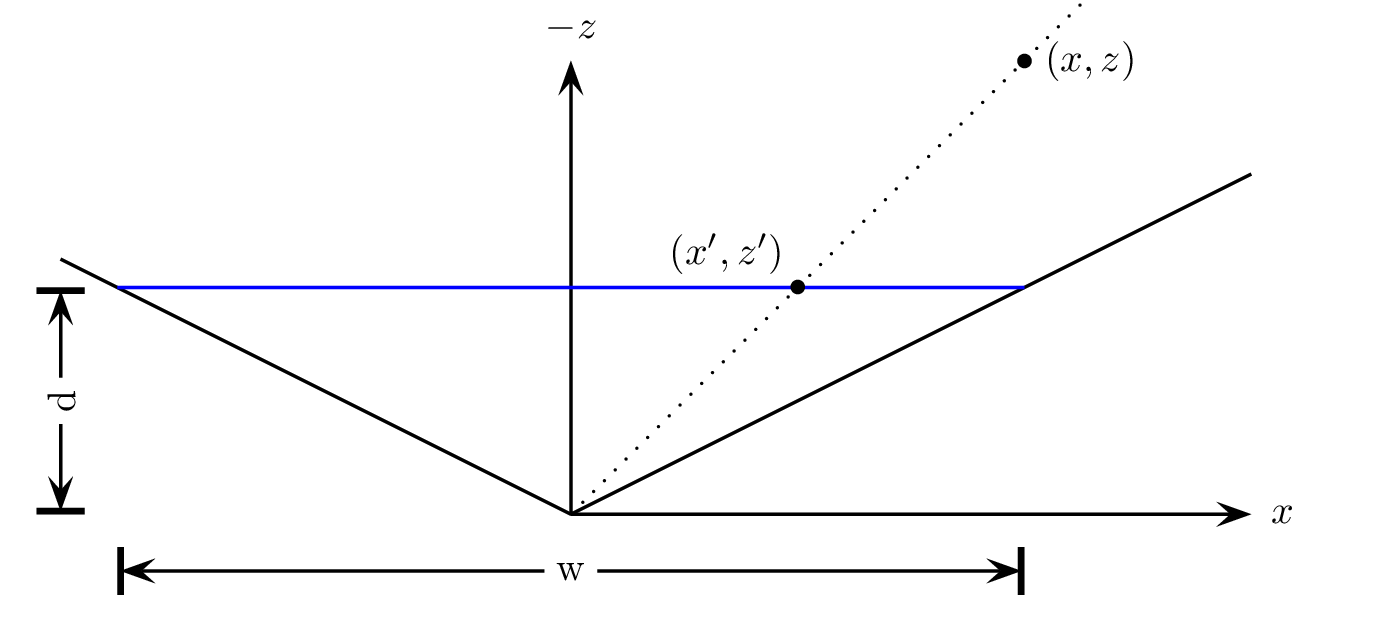
\includegraphics[width=\textwidth]{perspective.png}
\begin{itemize}
\item $z' = \pause -d$
\item $x' = \pause \frac{-xd}{z}$ because $\frac{x}{z} = \frac{x'}{z'}$
\item Scale $x'$ to $\pm 1$? $x' = \pause \frac{-2xd}{zw}$
\end{itemize}
\end{frame}

\sect{Simple Perspective Projection}
\begin{eqnarray*}
x' &=&  \frac{-2d}{zw}x\\
y' &=& \frac{-2d}{zh}y\\
z' &=&  -d\\
\mhomo{?&?&?&?}{?&?&?&?}{?&?&?&?} \phomo{x\\y\\z}&=&\phomo{x'\\y'\\z'}
\end{eqnarray*}
\begin{itemize}
\item What to do?
\end{itemize}
\end{frame}


\sect{Simple Perspective Projection}
\begin{eqnarray*}
x' &=&  \frac{-2d}{zw}x\\
y' &=& \frac{-2d}{zh}y\\
z' &=&  -d\\
\mhomo{\frac{-2d}{w}&0&0&0}
      {0&\frac{-2d}{h}&0&0}
      {0&0&0&-d} \phomo{x\\y\\z}
  &=&\phomo{\frac{-2xd}{w}\\\frac{-2yd}{h}\\-d}
\end{eqnarray*}
\begin{itemize}
\item Not quite there, we need to divide $x'$ and $y'$ by $z$.
\item How do we do that?
\item And {\em not} divide $z'$ by $z$?
\end{itemize}
\end{frame}

\sect{Simple Perspective Projection}
\begin{eqnarray*}
x' &=&  \frac{-2d}{zw}x\\
y' &=& \frac{-2d}{zh}y\\
z' &=&  -d\\
\mhomo{\frac{-2d}{w}&0&0&0}
      {0&\frac{-2d}{h}&0&0}
      {0&0&-d&0} \phomo{x\\y\\z}
  &=&\phomo{\frac{-2xd}{w}\\\frac{-2yd}{h}\\-dz}
\end{eqnarray*}
\begin{itemize}
\item Now we have to divide $x'$, $y'$ and $z'$ by $z$
\item How can we divide  by $z$?
\end{itemize}
\end{frame}

\sect{Simple Perspective Projection}
\begin{eqnarray*}
x' &=&  \frac{-2d}{zw}x\\
y' &=& \frac{-2d}{zh}y\\
z' &=&  -d\\
\wmhomo{\frac{-2d}{w}&0&0&0}
      {0&\frac{-2d}{h}&0&0}
      {0&0&-d&0}
      {0&0&1&0} \phomo{x\\y\\z}
  &=&\whomo{\frac{-2xd}{w}\\\frac{-2yd}{h}\\-dz\\z}
\end{eqnarray*}
\begin{itemize}
\item What point does this unhomogenized point represent?
\end{itemize}
\end{frame}

\sect{Simple Perspective Projection}
\begin{eqnarray*}
x' &=&  \frac{-2d}{zw}x\\
y' &=& \frac{-2d}{zh}y\\
z' &=&  -d\\
\wmhomo{\frac{-2d}{w}&0&0&0}
      {0&\frac{-2d}{h}&0&0}
      {0&0&-d&0}
      {0&0&1&0} \phomo{x\\y\\z}
  &=&\whomo{\frac{-2xd}{w}\\\frac{-2yd}{h}\\-dz\\z}\\
&=&\phomo{\frac{-2xd}{wz}\\\frac{-2yd}{hz}\\-d}\\
\end{eqnarray*}
\end{frame}

\sect{Simple Perspective Projection}
\begin{eqnarray*}
x' &=&  \frac{-2d}{zw}x\\
y' &=& \frac{-2d}{zh}y\\
z' &=&  -d\\
\wmhomo{\frac{2d}{w}&0&0&0}
      {0&\frac{2d}{h}&0&0}
      {0&0&d&0}
      {0&0&-1&0} \phomo{x\\y\\z}
  &=&\whomo{\frac{2xd}{w}\\\frac{2yd}{h}\\dz\\-z}\\
&=&\phomo{\frac{-2xd}{wz}\\\frac{-2yd}{hz}\\-d}\\
\end{eqnarray*}
\end{frame}

\sect{Problems projecting onto $z=-d$ plane.}
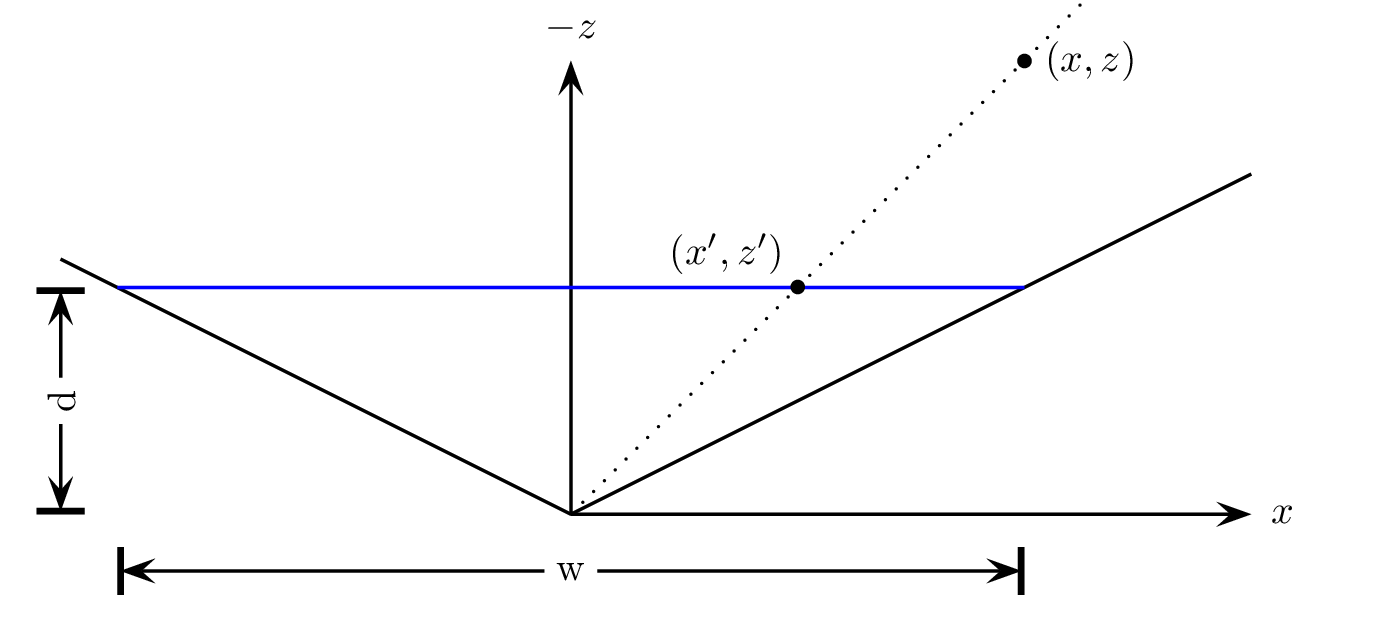
\includegraphics[width=1\textwidth]{perspective.png}
\begin{itemize}
\item If two items are on the same projection line, which one colors
  the image? 
\item We need to retain depth ($z$) information to decide.
\end{itemize}
\end{frame}

\sect{Problems projecting onto $z=-d$ plane.}
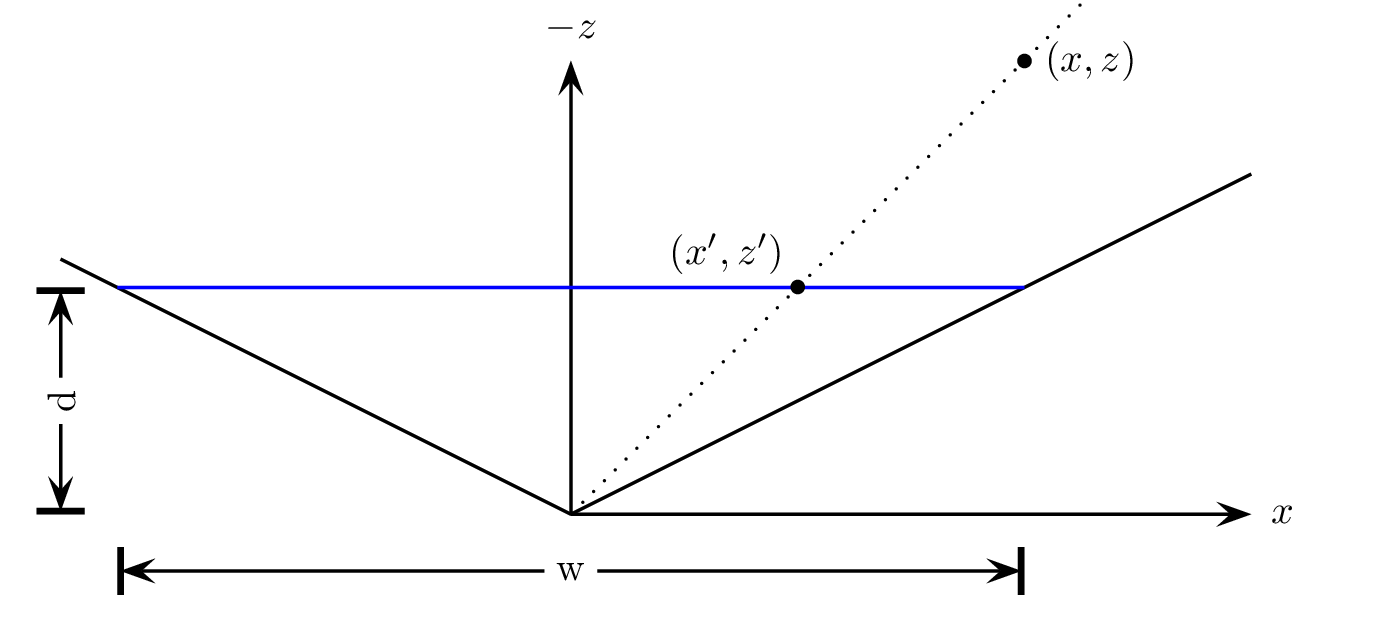
\includegraphics[width=1\textwidth]{perspective.png}
\begin{itemize}
\item {\bf Painter's algorithm:}  sort all objects and render them
  back to front.  This is an $O(n\log n)$ algorithm.
\end{itemize}
\end{frame}

\sect{Problems projecting onto $z=-d$ plane.}
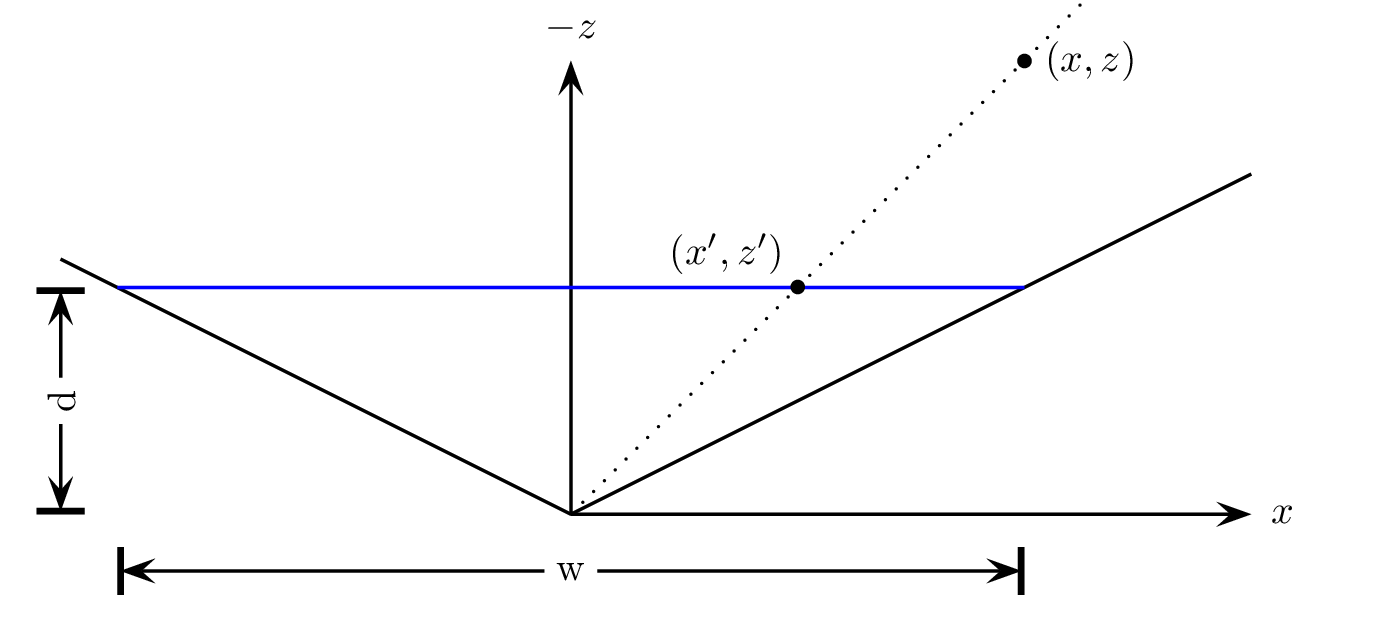
\includegraphics[width=1\textwidth]{perspective.png}
\begin{itemize}
\item {\bf Z-buffer algorithm:}  maintain a separate buffer where each
  item writes its depth.  Only if an item's depth is smaller than the
  depth already in the depth buffer does it write to the color buffer.
This is an $O(n)$ algorithm.
\end{itemize}
\end{frame}

\sect{Problems projecting onto $z=-d$ plane.}
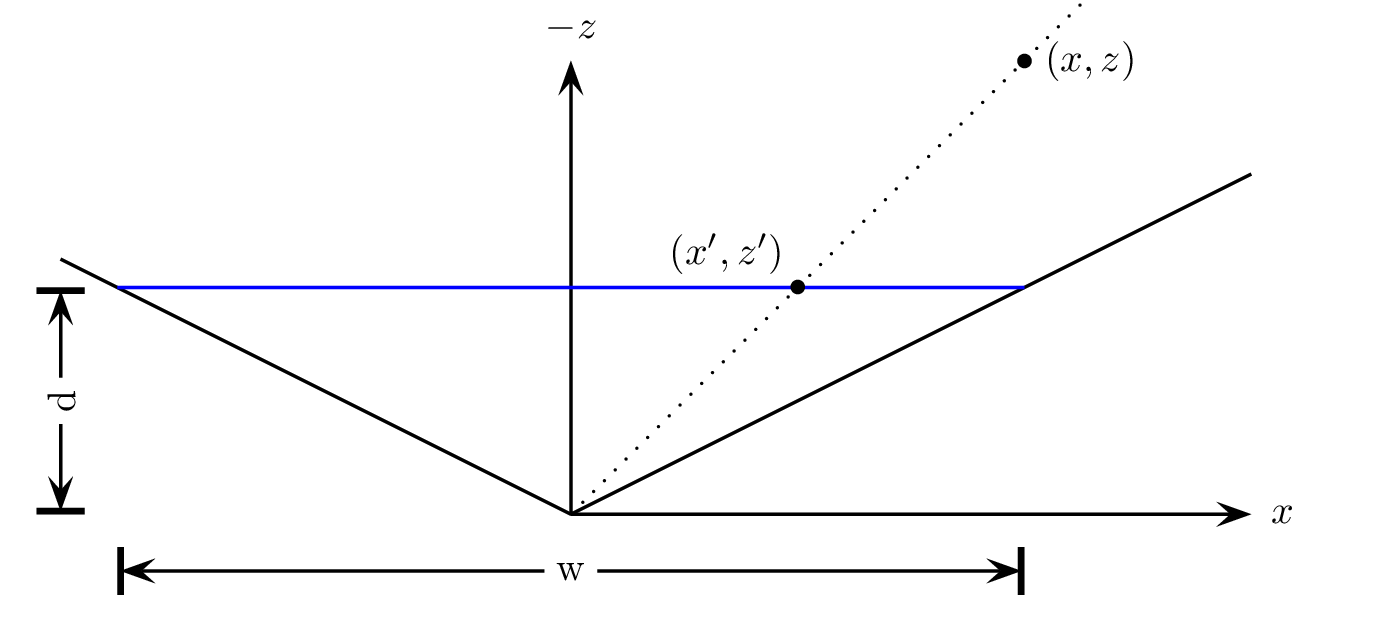
\includegraphics[width=1\textwidth]{perspective.png}
\begin{itemize}
\item We will retain the code to get $x'$ and $y'$ into the $\pm 1$
  cube, but instead of mapping $z$ to $-d$, we will map $z$ between
  {\em far} and {\em near} to $\pm 1$.
\item We will then use this depth in the z-buffer algorithm.
\end{itemize}
\end{frame}

\sect{Linear mapping between frames, one dimension}
\graphc{1}{onedlinear.png}
\begin{eqnarray*}
\mtwo{?}{?}{?}{?} \vtwo{p}{1} &=& \vtwo{p'}{1}\\
\pause
\mtwo{?}{?}{0}{1} \vtwo{p}{1} &=& \vtwo{p'}{1}\\
\pause
 c + \left(\frac{p-a}{b-a}\right)(d-c) &=& p'\\
\pause
\frac{d-c}{b-a}p + \frac{bc - ad}{b-a} &=& p'\\
\pause
\mtwo{\frac{d-c}{b-a}}{\frac{bc-ad}{b-a}}{0}{1}  \vtwo{p}{1} &=& \vtwo{p'}{1}
\end{eqnarray*}
\end{frame}

\sect{Linear mapping between frames, three dimensions}
\graphc{0.5}{threedlinear.png}
\pause
\begin{eqnarray*}
 c + \left(\frac{p-a}{b-a}\right)(d-c) &=& p'\\
\frac{d-c}{b-a}p + \frac{bc - ad}{b-a} &=& p'\\
\end{eqnarray*}
\end{frame}


\sect{Orthographic Projection in OpenGL}
\graphc{.9}{gl_projectionmatrix02.png}
\begin{itemize}
\item Map an arbitrary axially aligned bounding box (AABB) to
  normalized device coordinates (NDC), the $\pm 1$ cube.
\item $x$: $r \Rightarrow 1$\hspace{1cm}
 $l \Rightarrow -1$\\
\item $y$: $t \Rightarrow 1$\hspace{1cm}
 $b \Rightarrow -1$\\
\item $z$:  $f \Rightarrow 1$\hspace{1cm}
 $n \Rightarrow -1$
\end{itemize}
\end{frame}

\sect{Orthographic Projection in OpenGL}
\graphc{1}{onedlinear.png}
\begin{itemize}
\item Map $x$ between $l$ and $r$ to between $-1$ and $+1$
\end{itemize}
\begin{eqnarray*}
x' &=& \frac{d-c}{b-a}x + \frac{bc - ad}{b-a} \\\pause
   &=& \frac{1-(-1)}{r-l}x + \frac{-r-l}{r-l}\\
    &=& \frac{2}{r-1}x - \frac{r+l}{r-l}\\
y' &=& \frac{2}{t-b}y - \frac{t+b}{t-b}\\
z' &=& \frac{-2}{f-n}z - \frac{f+n}{f-n}
\end{eqnarray*}
\end{frame}

\sect{Orthographic Projection in OpenGL}
\graphc{.9}{gl_projectionmatrix02.png}
\begin{eqnarray*}
\mhomo
{\frac{2}{r-l} & 0 & 0 & -\frac{r+l}{r-l}}
{0 & \frac{2}{t-b} & 0 & -\frac{t+b}{t-b}}
{0 & 0 & \frac{-2}{f-n} & -\frac{f+n}{f-n}}
\phomo{x\\y\\z} 
&=&
\phomo{x'\\y'\\z'}
\end{eqnarray*}
\begin{itemize}
\item If symmetric around $z$-axis, $r=-l$ and $t=-b$.
\end{itemize}
\end{frame}

\sect{Orthographic Projection in OpenGL}
\graphc{.9}{gl_projectionmatrix02.png}
\begin{itemize}
\item If symmetric around $z$-axis, $r=-l$ and $t=-b$, then
\end{itemize}
\begin{eqnarray*}
\mhomo
{\frac{1}{r} & 0 & 0 & 0}
{0 & \frac{1}{t} & 0 & 0}
{0 & 0 & \frac{-2}{f-n} & -\frac{f+n}{f-n}}
\phomo{x\\y\\z} 
&=&
\phomo{x'\\y'\\z'}
\end{eqnarray*}
\end{frame}


\sect{Projective Transforms in OpenGL}
\graphc{1}{gl_projectionmatrix01.png}
\begin{itemize}
\item Map an arbitrary view frustrum to
  normalized device coordinates (NDC), the $\pm 1$ cube.
\end{itemize}
\end{frame}

\sect{Projective Transforms in OpenGL}
\graph{.49}{gl_projectionmatrix03.png}\hfill
\graph{.49}{gl_projectionmatrix04.png}
\begin{itemize}
\item Find the $x$ and $y$ coordinates using similar triangles.
\end{itemize}
\begin{eqnarray*}
x' &=& -\frac{n}{z}x\\
y' &=& -\frac{n}{z}y
\end{eqnarray*}
\end{frame}

\sect{Projective Transforms in OpenGL}
\begin{itemize}
\item It looks like dividing by $-z$ is going to be a good idea again,
  so let's fill in the bottom row of our matrix.
\end{itemize}
\begin{eqnarray*}
x' &=& -\frac{n}{z}x\\
y' &=& -\frac{n}{z}y
\end{eqnarray*}\pause
\[\wmhomo{?&?&?&?}{?&?&?&?}{?&?&?&?}{0&0&-1&0}\phomo{x\\y\\z}
=\whomo{x_u\\y_u\\z_u\\-z}
=\phomo{x'\\y'\\z'}
\]
\end{frame}

\sect{Projective Transforms in OpenGL}
\graphc{.8}{gl_projectionmatrix01.png}
\begin{itemize}
\item Now we map $x$ and $y$ to normalized device coordinates, as
  before: 
\begin{eqnarray*}
 x' &=& \left(\frac{2}{r-l}\right)\left(-\frac{n}{z}x\right)-\frac{r+l}{r-l}\\
\pause
 &=& \left[\left(\frac{2n}{r-l}\right)x + \left(\frac{r+l}{r-l}\right)z\right]/(-z)
\end{eqnarray*}
\end{itemize}
\end{frame}


\sect{Projective Transforms in OpenGL}
\begin{itemize}
\item Now we can get more rows of our matrix.
\end{itemize}
\begin{eqnarray*}
 x'  &=& \left[\left(\frac{2n}{r-l}\right)x
      + \left(\frac{r+l}{r-l}\right)z\right]/(-z)
\end{eqnarray*}
\begin{eqnarray*}
\wmhomo
{?&?&?&?}
{?&?&?&?}
{?&?&?&?}
{0&0&-1&0}
\phomo{x\\y\\z}
&=&\whomo{x_u\\y_u\\z_u\\-z}
=\whomo{x'\\y'\\z'\\1}\\
\pause
\wmhomo
{\frac{2n}{r-l}& 0 & \frac{r+l}{r-l}& 0}
{0 & \frac{2n}{t-b}&\frac{t+b}{t-b}& 0}
{?&?&?&?}
{0&0&-1&0}
\phomo{x\\y\\z}
&=&\whomo{x_u\\y_u\\z_u\\-z}
=\whomo{x'\\y'\\z'\\1}\\
  \end{eqnarray*}
\end{frame}

\sect{Projective Transforms in OpenGL}
\begin{itemize}
\item Finding the third row of our matrix.
\item We know $z'$ does not depend on $x$ or $y$, so let's try this:
\begin{eqnarray*}
\wmhomo
{\frac{2n}{r-l}& 0 & \frac{r+l}{r-l}& 0}
{0 & \frac{2n}{t-b}&\frac{t+b}{t-b}& 0}
{0&0&A&B}
{0&0&-1&0}
\phomo{x\\y\\z}
&=&\whomo{x_u\\y_u\\z_u\\-z}
=\phomo{x'\\y'\\z'}
  \end{eqnarray*}
\[
z' =\frac{Az + B}{-z}
\]
\item Now solve for $A$ and $B$
\end{itemize}
\end{frame}

\sect{Projective Transforms in OpenGL}
\graphc{.8}{gl_projectionmatrix01.png}
\[
z' =\frac{Az + B}{-z}
\]
\pause
\begin{itemize}
\item When $z = -n$, $z' = -1$
\item When $z = -f$, $z' = +1$
\end{itemize}
\end{frame}

\sect{Projective Transforms in OpenGL}
\[
z' =\frac{Az + B}{-z}
\]
\begin{itemize}
\item When $z = -n$, $z' = -1$
\item When $z = -f$, $z' = +1$
\end{itemize}
\begin{eqnarray*}
-1 &=& \frac{-nA+B}{n}\\
1 &=& \frac{-fA+B}{f}\\
A &=& -\frac{f+n}{f-n}\\
B &=& -\frac{2fn}{f-n}
\end{eqnarray*}
\end{frame}

\sect{Projective Transforms in OpenGL}
\graphc{.8}{gl_projectionmatrix01.png}
\begin{eqnarray*}
\wmhomo
{\frac{2n}{r-l}& 0 & \frac{r+l}{r-l}& 0}
{0 & \frac{2n}{t-b}&\frac{t+b}{t-b}& 0}
{0&0& -\frac{f+n}{f-n}& -\frac{2fn}{f-n}}
{0&0&-1&0}
\phomo{x\\y\\z}
&=&\whomo{x_u\\y_u\\z_u\\-z}
=\phomo{x'\\y'\\z'}
  \end{eqnarray*}
\end{frame}

\sect{Projective Transforms in OpenGL}
\graphc{.8}{gl_projectionmatrix01.png}
\begin{itemize}
\item When symmetric, $r=-l$ and $t=-b$, it simplifies:
\end{itemize}
\begin{eqnarray*}
\wmhomo
{\frac{n}{r}& 0 & 0& 0}
{0 & \frac{n}{t}&0& 0}
{0&0& -\frac{f+n}{f-n}& -\frac{2fn}{f-n}}
{0&0&-1&0}
\phomo{x\\y\\z}
&=&\whomo{x_u\\y_u\\z_u\\-z}
=\phomo{x'\\y'\\z'}
  \end{eqnarray*}
\end{frame}


\sect{Z fighting in OpenGL}
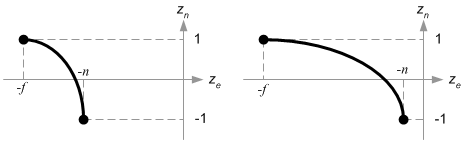
\includegraphics[width=\textwidth]{gl_projectionmatrix07.png}
\begin{eqnarray*}
z' &=& \frac{f+n}{f-n} + \frac{2fn}{z(f-n)}
\end{eqnarray*}
\end{frame}

\end{document}
